% Ana y Alexander:
% Aqui esta la presentacion de python, ya estan todos los temas en
% la tabla de contenidos, la idea de esto es que podamos aprender
% de openCv y latex al tiempo.
%
% Para poder terminar la presentacion se necesitan varias cosas
%
%     1) Agreguen su nombre a los autores (reemplacen en donde dice !nombres!)
%     2) Por favor completar los frames que estan en blanco
%     3) Por favor dar ejemplos en los que se usen las colecciones,
%        clases y herencia
%
% Para que les sea mas facil buscar la informacion en drive esta el libro en
% el que me base para hacer los ejemplos. Se llama Python para todos,
% pero el archivo es un link al libro en si, esta en la carpeta 2016/Libros
%
% Con ese libro tienen para sacar toda la informacion
%
% Muchas gracias

\documentclass{beamer}
\usepackage{graphicx}
\usepackage{listings}
\usepackage{enumerate}
%\usepackage[spanish]{babel}

\begin{document}

\title{Python Katas}
    \author{Alexander Acosta Jim\'enez \\
            Ana Mar\'ia Bedoya Hern\'andez \\}
    \date{\today}

    \frame{ \titlepage }
    
    \frame{
    \frametitle{Tabla de contenidos}

    \begin{enumerate}
        \item Diferencia entre Git y GitHub
 	    \item Servidores de repositorios Git
        \item Instalar Git
        \item C\'omo crear un repositorio?
	   \item Los tres estados

	  %\item Principales conceptos
        \item C\'omo compartir un repositorio?
        \item Committing, Pull y Push
        \item C\'omo crear un Brach?
        \item Merging
    \end{enumerate}
}

    \begin{frame}[fragile]
  \frametitle{Introducci\'on a Python}
  
  \begin{itemize}
  \item Qu\'e es Python?
  \item Caracter\'isticas
    \begin{itemize}
      
    \item Lenguaje interpretado
      
    \item Tipado din\'amico
      
    \item Fuertemente tipado
      
    \item Multiplataforma
      
    \item Orientado a objetos
      
    \end{itemize}
    
  \end{itemize}

  
  \begin{figure}
    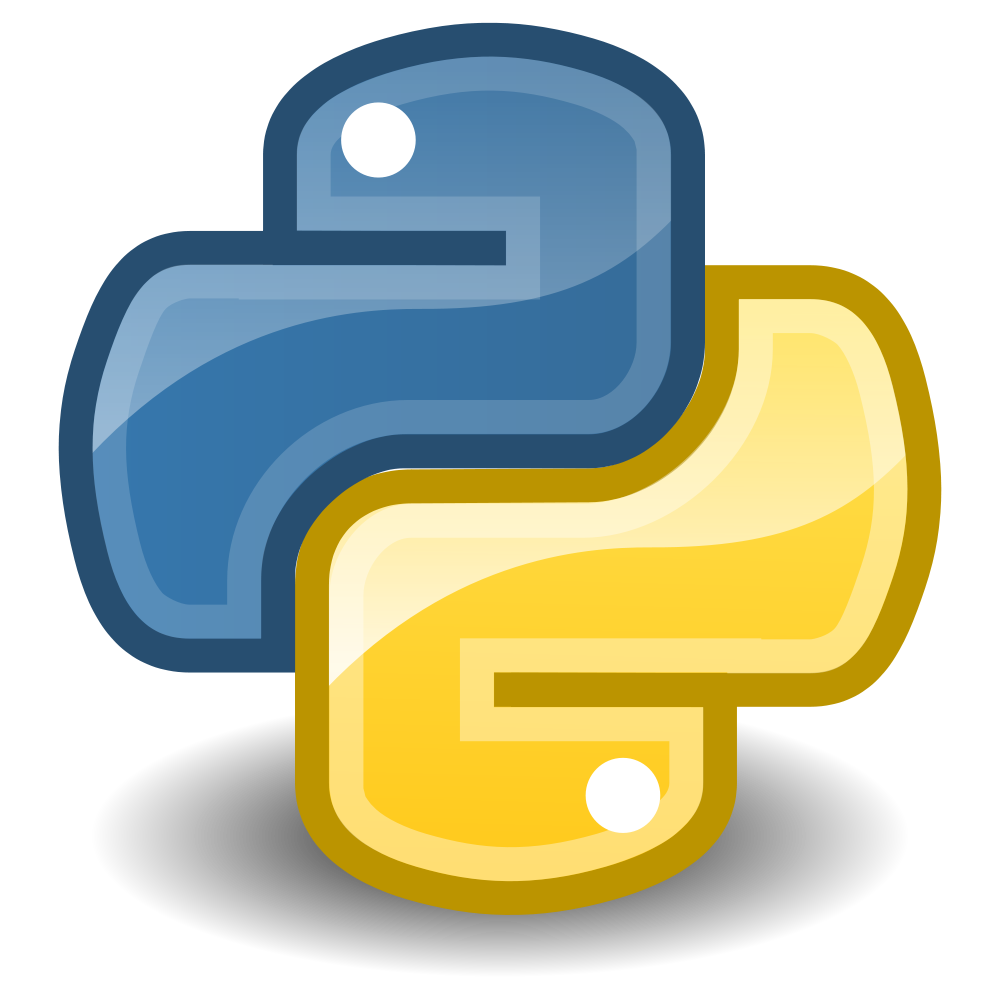
\includegraphics[width=0.3\textwidth]{Imagenes/Python.jpg}
  \end{figure}

\end{frame}

    \begin{frame}[fragile]
    \frametitle{Tipos b\'asicos}

    Al igual que en cualquier lenguaje de programaci\'on Python tiene
    tipos b\'asicos como:

    \begin{itemize}
        \item Num\'erico
            \begin{itemize}
                \item Entero
                \item Flotante
            \end{itemize}
        \item Cadenas
        \item Booleanos
    \end{itemize}

    Por inferencia de tipos en Python se pueden definir variables de la
    siguiente manera:

    \lstset{ morecomment=[l][\color{blue}]{\#} }
    \begin{lstlisting}
    entero = 1
    flotante = 1.2
    cadena = "cadena"
    booleano = True
    \end{lstlisting}

\end{frame}

    \begin{frame}[fragile]
  \frametitle{Colecciones}

  En Python existen tres tipos de colecciones:

  \begin{enumerate}[1.]
    \item Listas
    \item Tuplas
    \item Diccionarios
  \end{enumerate}
  
  
\end{frame}


    \begin{frame}[fragile]
  \frametitle{Colecciones}

  \begin{enumerate}[1.]
    \item Listas    
  \end{enumerate}


  La lista es un tipo de colecci\'on ordenada, es equivalente  a lo que en otros lenguajes se conoce como arrays o vectores. Pueden contener cualquier tipo de dato: n\'umeros, cadenas,
booleanos, ... y tambi\'en listas.

  \begin{itemize}
    \item Ejemplo:
  \end{itemize}

  \begin{figure}
    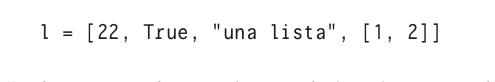
\includegraphics[width=0.6\textwidth]{Imagenes/Listas.jpg}
    \caption{\label{fig:Ejemplo1}Creaci\'on de una lista en Python.}
  \end{figure}  
 
 
\end{frame}


    \begin{frame}[fragile]
  \frametitle{Colecciones}

  \begin{enumerate}[2.]
    \item Tuplas    
  \end{enumerate}


  Una tupla es una lista inmutable, es decir, no puede modificarse de ning\'un modo despu\'es de su creaci\'on. Se define igual que una lista, salvo que el conjunto se encierra entre par\'entesis en lugar de entre corchetes. Tambi\'en tienen un orden definido.

  \begin{itemize}
    \item Ejemplo:
  \end{itemize}

  \begin{figure}
    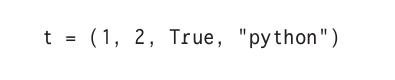
\includegraphics[width=0.6\textwidth]{Imagenes/Tuplas.jpg}
    \caption{\label{fig:Ejemplo2}Creaci\'on de una tupla en Python.}
  \end{figure}  
 
 
\end{frame}

    \begin{frame}[fragile]
  \frametitle{Colecciones}

  \begin{enumerate}[3.]
    \item Diccionarios    
  \end{enumerate}

  Los diccionarios deben su nombre a que son colecciones que relacionan una clave y un valor. El primer valor se trata de la clave y el segundo del valor asociado a la clave. La diferencia principal entre los diccionarios y las listas o las tuplas es que se accede a su valor por medio de su clave usando corchetes.

  \begin{itemize}
    \item Ejemplo:
  \end{itemize}

  \begin{figure}
    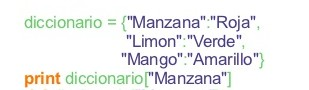
\includegraphics[width=0.6\textwidth]{Imagenes/Diccionarios.jpg}
    \caption{\label{fig:Ejemplo3}Creaci\'on de un diccionario en Python.}
  \end{figure}  
 
 
\end{frame}

    \begin{frame}[fragile]
  \frametitle{Control de flujo}

    \framesubtitle{Sentencias condicionales}    

  \begin{itemize}
    \item Sentencia if
  \end{itemize}

  \begin{figure}
    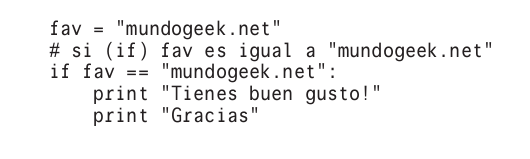
\includegraphics[width=0.6\textwidth]{Imagenes/If.jpg}
    \caption{\label{fig:Ejemplo4}Sintaxis de if en Python.}
  \end{figure}

\end{frame}

  

    \begin{frame}[fragile]
  \frametitle{Control de flujo}

    \framesubtitle{Sentencias condicionales}    
  
  \begin{itemize}
    \item Sentencia if...else
  \end{itemize}

  \begin{figure}
    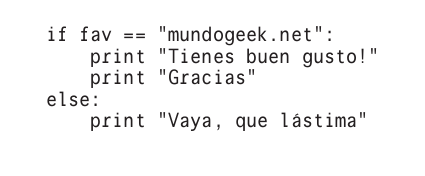
\includegraphics[width=0.6\textwidth]{Imagenes/IfElse.jpg}
    \caption{\label{fig:Ejemplo5}Sintaxis de if...else en Python.}
  \end{figure}

\end{frame}

    \begin{frame}[fragile]
  \frametitle{Control de flujo}

    \framesubtitle{Sentencias condicionales}    


  \begin{itemize}
    \item Sentencia if...elif
  \end{itemize}

  \begin{figure}
    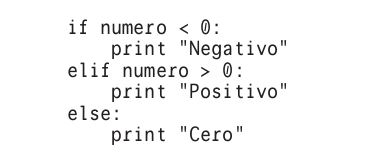
\includegraphics[width=0.6\textwidth]{Imagenes/IfElif.jpg}
    \caption{\label{fig:Ejemplo6}Sintaxis de if...elif en Python.}
  \end{figure}

\end{frame}

    \begin{frame}[fragile]
  \frametitle{Control de flujo}

    \framesubtitle{Bucles}    
  
  \begin{itemize}
    \item Ciclo while
  \end{itemize}

  El bucle while(Mientras) ejecuta un fragmento de c\'odigo mientras se cumpla una condici\'on.

  \begin{figure}
    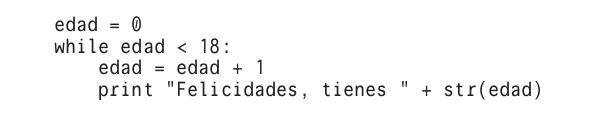
\includegraphics[width=0.6\textwidth]{Imagenes/While.jpg}
    \caption{\label{fig:Ejemplo7}Sintaxis de while en Python.}
  \end{figure}

\end{frame}


    \begin{frame}[fragile]
  \frametitle{Control de flujo}

    \framesubtitle{Bucles}    

  \begin{itemize}
    \item Ciclo for...in
  \end{itemize}

  El ciclo for se utiliza como una forma gen\'erica de iterar sobre una secuencia.

  \begin{figure}
    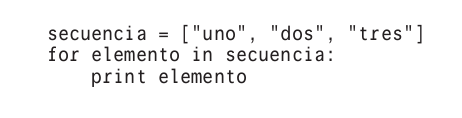
\includegraphics[width=0.6\textwidth]{Imagenes/For.jpg}
    \caption{\label{fig:Ejemplo8}Sintaxis de for...in en Python.}
  \end{figure}

\end{frame}

    \begin{frame}[fragile]
  \frametitle{Funciones}

  Una funci\'on es un fragmento de c\'odigo con un nombre asociado que
  realiza una serie de tareas y devuelve un valor.

  \begin{itemize}
  \item{Ejemplo:}
  \end{itemize}
  
  \begin{figure}
    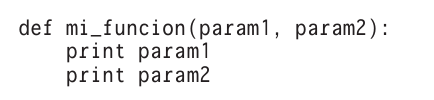
\includegraphics[width=0.6\textwidth]{Imagenes/Ejm.jpg}
    \caption{\label{fig:Ejm}Esta funci\'on imprime los dos par\'ametros ingresados.}
  \end{figure}

\end{frame}

    \begin{frame}[fragile]
  \frametitle{Clases y objetos}
  
  Una clase no es m\'as que una plantilla gen\'erica a partir de la cual se pueden instanciar objetos;
  en esta plantilla es donde se definen qu\'e atributos y m\'etodos tendr\'an los objetos de esa clase.
  
  \begin{figure}
    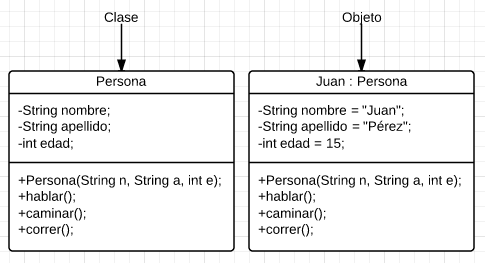
\includegraphics[width=0.6\textwidth]{Imagenes/ClaseObjeto.jpg}
    % \caption{\label{fig:Ejm}Esta funci\'on imprime los dos parametros ingresados.}
  \end{figure}
  
\end{frame}


    \begin{frame}[fragile]
  \frametitle{Clases y objetos}

  \begin{itemize}
  \item{Ejemplo:}
  \end{itemize}
  
  
  \begin{figure}
    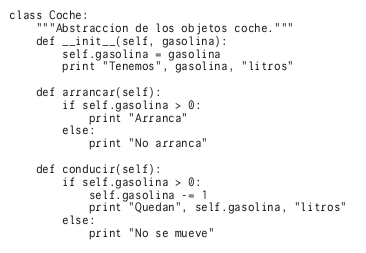
\includegraphics[width=0.6\textwidth]{Imagenes/Ejm2.jpg}
    % \caption{\label{fig:Ejm}Esta funci\'on imprime los dos parametros ingresados.}
  \end{figure}
  
\end{frame}

    \begin{frame}[fragile]
  \frametitle{Herencia}


  La herencia sirve para crear clases nuevas a partir de clases preexistentes.
  Se heredan atributos y m\'etodos de las clases viejas  para modelar una nueva situaci\'on.
   
\end{frame}

    \begin{frame}[fragile]
  \frametitle{Herencia}
  
  \begin{itemize}
  \item{Ejemplo:}
  \end{itemize}
  
  
  \begin{figure}
    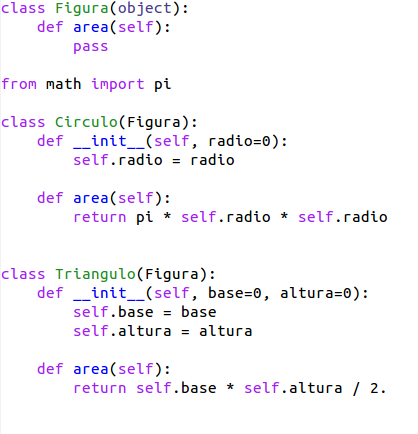
\includegraphics[width=0.6\textwidth]{Imagenes/EjmH.png}
    % \caption{\label{fig:EjmH}Esta funci\'on imprime los dos parametros ingresados.}
  \end{figure}
  
\end{frame}

    \begin{frame}[fragile]
  \frametitle{M\'odulos y paquetes}

  \framesubtitle{M\'odulos}

  Para facilitar el mantenimiento y la lectura, los programas demasiado largos pueden dividirse en m\'odulos, agrupando elementos relacionados.

  \begin{figure}
    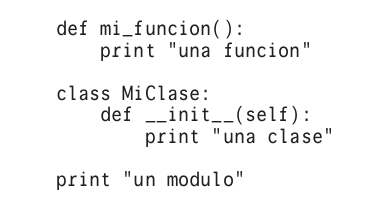
\includegraphics[width=0.6\textwidth]{Imagenes/Modulo.jpg}
    \caption{\label{fig:Ejemplo9}Ejemplo de un m\'odulo en Python.}
  \end{figure}

 

\end{frame}

    \begin{frame}[fragile]
  \frametitle{M\'odulos y paquetes}

  \framesubtitle{M\'odulos}

  Si se quisiera utilizar la funcionalidad definida en el m\'odulo anterior en nuestro programa se necesita importarlo.

  \begin{figure}
    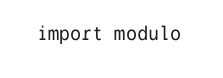
\includegraphics[width=0.6\textwidth]{Imagenes/Import.jpg}
    \caption{\label{fig:Ejemplo11}Sintaxis de import en Python.} 
  \end{figure}

  El import no solo hace que tengamos disponible todo lo definido dentro del m\'odulo, sino que tambi\'en ejecuta el c\'odigo dentro de \'el. 

\end{frame}

    \begin{frame}[fragile]
  \frametitle{M\'odulos y paquetes}

  \framesubtitle{Paquetes}

  Si los m\'odulos sirven para organizar el c\'odigo, los paquetes sirven para organizar los m\'odulos. Los paquetes son tipos especiales de m\'odulos (ambos son de tipo module) que permiten agrupar m\'odulos relacionados.Se representan mediante directorios.

  \begin{figure}
    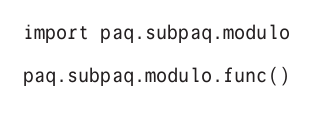
\includegraphics[width=0.6\textwidth]{Imagenes/Paquetes.jpg}
    \caption{\label{fig:Ejemplo12}Ejemplo de paquetes en Python.}
  \end{figure}

 

\end{frame}

    \begin{frame}[fragile]
  \frametitle{Bibliograf\'ia}

  \begin{itemize}
    \item Libro: Python para Todos. Autor: Ra\'ul G\'onzalez Duque.
  \end{itemize}

\end{frame}


\end{document}
